\ifdefined\MAINDOC\else
\documentclass[10pt, a4paper, fleqn]{article}
\usepackage{base}

\begin{document}
    \title{Skript Mathe 2}
    \date{13. Juni 2018}
    \maketitle
\fi
\subsection{Bemerkung}
Wegen 5.28 ist $e \approx 2,718$ die Basis zur Exponentialfunktion $\exp(x)$. \\
Man erhält $e^x = \underset{\text{4.11a2}}{\exp}(x \cdot \ln(\underset{= \exp(1)}{e})) = \exp(x)$

Siehe auch 4.11 Exkurs

\subsection{Minimax-Theorem von Weierstraß}

Jede stetige Funktion $f: [a, b] \to \IR$ besitzt sowohl ein Minimum als auch ein Maximum,
d.h:
\[
    \exists x_*, x^* \in [a, b]: f(x_*) \leq f(x) \leq f(x^*) \quad \forall x \in [a, b]    
\]
\textbf{Beweis: } Genügt z.Z: $f$ hat Maximum (Minimum analog).

Sei $s := \sup f([a, b])$ (kleinste obere Schranke des Bildes von $f$).

Zeige: $s < \infty$ und $s \in f([a, b])$.

Sei $(X_n)$ Folge in $[a, b]$ mit $f(X_n) \to s$.

$(X_n)$ beschränkt $\imp \exists$ konvergente Teilfolge $(X_{n_j})$ mit
$\lim\limits_{i \to \infty} X_{n_j} = \tilde{x}, \tilde{x} \in [a, b]$, da
$[a, b]$ abgeschlossen, ist $f$ stetig.

$\imp \lim\limits_{j \to \infty} f(X_{n_j}) = s = f(\tilde{x})$ \\
$\imp s$ Funktionswert von $\tilde{x}$ und somit $f < \infty$ \\
$\imp s \in f([a, b])$ und somit $f(x) \leq s \quad \forall x \in [a, b]$

\subsection{Beispiele}
\begin{enumerate}[a)]
    \item $f(x) = x^2$ auf $[0, 1]$ \\
    $f(x_*) = 0, f(x^*) = 1$

    \item Falls der Definitionsbereich nicht abgeschlossen ist:
    \begin{itemize}
        \item $f(x) = x^2$ besitzt auf $(0, 1)$ weder Minimum noch Maximum.
        \item $f(x) = \frac{1}{x}$ besitzt auf $(0, 1)$ weder Minimum noch Maximum,
        jedoch ist $f(\underbrace{x_*}_{1}) = 1$
    \end{itemize}
    \item $f(x) = \sin(x)$ hat je nach Größe des festgelegten Definitionsbereiches mehrere
    Minimal/-Maximalstellen
\end{enumerate}

\section{Differenzierbare Funktionen}

\subsection{Bemerkung: Tangenten}

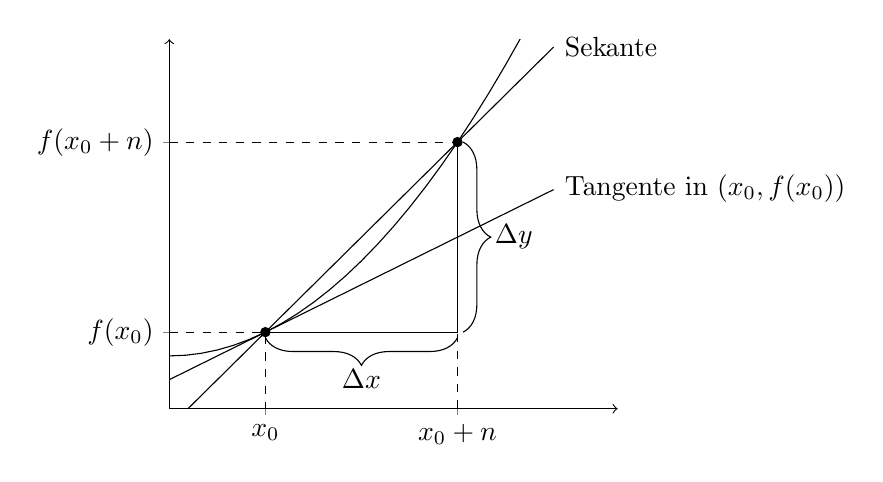
\begin{tikzpicture}[
    declare function = {
        f(\x) = \x^2 + 5;
        t(\x) = 3*x + 2.75;
        s(\x) = 6*x - 1.75;
    }
]
    \begin{axis}[
        width = 0.6\textwidth,
        axis x line = center,
        axis y line = left,
        ymin = 0, ymax = 35,
        xmin = 0, xmax = 7,
        xtick = {1.5, 4.5},
        xticklabels = {$x_0$, $x_0 + n$},
        ytick = {7.25, 25.25},
        yticklabels = {$f(x_0)$, $f(x_0 + n)$},
        axis line style = {->},
        domain = 0:6
    ]
    \addplot[color = black] {f(x)};  
    \addplot[color = black] {t(x)};
    \addplot[color = black] {s(x)};

    \draw (1.5, {f(1.5)}) node[circle, fill = black, scale = 0.4]{};
    \draw (4.5, {f(4.5)}) node[circle, fill = black, scale = 0.4]{};
    \draw (1.5, {f(1.5)}) -- (4.5, {f(1.5)}) -- (4.5, {f(4.5)});
    
    \draw[dashed] (0, {f(1.5)}) -- (1.5, {f(1.5)}) -- (1.5, 0);
    \draw[dashed] (0, {f(4.5)}) -- (4.5, {f(4.5)});
    \draw[dashed] (4.5, 0) -- (4.5, {f(1.5)});

    \draw[decorate, decoration = {brace, amplitude = 10pt, raise = 2pt}] 
        (4.5, {f(1.5)}) -- (1.5, {f(1.5)}) node[midway, below = 10pt]{$\Delta x$};
    \draw[decorate, decoration = {brace, amplitude = 10pt, raise = 2pt}] 
        (4.5, {f(4.5)}) -- (4.5, {f(1.5)}) node[midway, right = 10pt]{$\Delta y$};

    \end{axis}
    \draw (4.9, 2.8) node[right] {Tangente in $(x_0, f(x_0))$};
    \draw (4.9, 4.6) node[right] {Sekante};
\end{tikzpicture}

Die Sekante durch die Punkte $(x_0, f(x_0))$ und \\
$(x_0 + h, f(x_0 + h))$ hat die Steigung 
\[
    \frac{\Delta x}{\Delta y} =
    \frac{f(x_0 + h) - f(x_0)}{h} \ \widehat{=} \text{ Differenzenquotient}
\]
Je kleiner $h$, desto besser nähert sich die Sekante an die Tangente
$(x_0, f(x_0))$ an. Daraus ergibt sich die Tangentensteigung:
$\lim\limits_{h \to 0} \dfrac{f(x_0 + h) - f(x_0)}{h}$, falls der Grenzwert existiert.

\bigskip
In diesem Kapitel sei $I$ immer offenes Intervall.
\subsection{Definition: Ableitung}
Sei $f: I \to \IR, x \in I$
\begin{enumerate}[1.]
    \item $f$ heißt differenzierbar in $x_0$, falls
    $\lim\limits_{h \to 0} \dfrac{f(x_0 + h) - f(x_0)}{h}$ existiert. Dieser
    Grenzwert heißt die Ableitung von $f$ in $x_0$ und wird mit $f'(x_0)$ oder
    $\dfrac{d}{dx} f(x_0)$ bezeichnet.

    \item Ist $f$ differenzierbar in jedem $x_0 \in I$, so heißt $f$ differenzierbar
    (auf $I$) und man nennet $f': I \to \IR, x \mapsto f'(x)$ die Abbildung von $f$.
\end{enumerate}

\subsection{Bemerkung}

Setzt man in 6.2/1 $x = x_0 + h$, so erhält man für den Grenzwert des
Differenzenquotienten $\lim\limits_{x \to x_0} \dfrac{f(x) - f(x_0)}{x - x_0}$.

\subsection{Beispiele}

\begin{enumerate}[a)]
    \item $f(x) = c$ für $x \in \IR$:
    \[
        \lim_{h \to 0} \frac{c - c}{h} = 0 = f'(x) \quad \forall x \in \IR
    \]

    \item $(x^2)' = 2x \quad \forall x \in \IR:$
    \[
        \frac{(x + h)^2 - x^2}{h} = \frac{\cancel{x^2} + 2x\bcancel{h} + h^2 - \cancel{x^2}}{\bcancel{h}} = 2x + h \to 2x
    \]

    \item $(x^n)' = nx^{n-1} \quad \forall x \in \IR, n \in \IN:$
    \[\begin{aligned}
        &\frac{(x + h)^n - x^n}{h} = \frac{\sum_{k=0}^n \qt{\binom{n}{k} x^{n - k} h^k} - x^n}{h} \\
        &= \sum_{k=1}^n \qt{\binom{n}{k} x^{n - k} h^{k-1}} - \underbrace{x^n}_{\mathclap{\substack{\to 0 \text{ für } \\ h \to 0, \ k \neq 1}}} \\
        &\to nx^{n-1} \text{ für } h \to 0
    \end{aligned}\]

    \item $\qt{\frac{1}{x}}' = -\frac{1}{x^2} \quad \forall x \neq 0:$
    \[\begin{aligned}
        &\frac{\frac{1}{x+h} - \frac{1}{x}}{h} = \frac{x - (x + h)}{(x + h)x \cdot h}
        = \frac{-1}{x \cdot (x + h)} \\
        &\to -\frac{1}{x^2} \text{ für } h \to 0
    \end{aligned}\]

    \item Analog zu c) erhält man
    \[
        \qt{\frac{1}{x^n}}' = \frac{-n}{x^{n+1}} \quad \forall x \neq 0    
    \]

    \item $(e^x)' = e^x$.

    Es ist $e^x = \exp(x)$ (5.29). Wir benutzen in Beweis von 5.28 \\
    $\lim\limits_{h \to 0} \dfrac{\exp(h) - 1}{h} = 1$. Damit gilt:
    \[\begin{aligned}
        &\frac{\exp(x + h) - \exp(x)}{h} = \frac{\exp(x) \exp(h) - \exp(x)}{h} \\
        & = \exp(x) \cdot \frac{\exp(h) - 1}{h} \xrightarrow[h \to 0]{} \exp(x)
    \end{aligned}\]

    \item $(\sin x)' = \cos(x), \ (\cos x)' = \sin(x) \quad \forall x \in \IR$

    Ohne Beweis. Man zeigt dies, indem man $\sin$ und $\cos$ mit Hilfe von $\exp$ darstellt
    ($\to$ Mathe III)
\end{enumerate}

\subsection{Satz: Lineare Approximation}

Sei $f: I \to \IR, x_0 \in I$.

Dann sind äquivalent:
\begin{enumerate}[1.]
    \item $f$ ist in $x_0$ differenzierbar
    \item Es gibt eine Funktion $R: I \to \IR$, stetig in $x_0$, $R(x_0) = 0$ und ein
    $m \in \IR$, so dass
    \[
        f(x) = f(x_0) + \underbrace{m(x - x_0)}_{\mathclap{\text{Tangente an $f$ in $x_0$}}}
        + R(x)(x - x_0) \quad (*)    
    \]
\end{enumerate}

Bemerkung: \begin{itemize}
    \item In $\IR: m = f'(x_0)$
    \item 2. heißt: $f$ ist in $x_0$ durch eine Gerade (Tangente) approximierbar.
\end{itemize}

\ifdefined\MAINDOC\else
\end{document}
\fi